\chapter{Iteración}

Este capítulo trata sobre la iteración, que es la capacidad de ejecutar un bloque de declaraciones repetidamente. Vimos un tipo de iteración, usando recursión, en la Sección 5.8. Vimos otro tipo, usando un bucle \texttt{for}, en la Sección 4.2. En este capítulo veremos otro tipo más, usando una declaración \texttt{while}. Pero primero quiero decir un poco más sobre la asignación de variables.

\section{Reasignación}

Como puedes haber descubierto, es legal hacer más de una asignación a la misma variable. Una nueva asignación hace que una variable existente se refiera a un nuevo valor (y deje de referirse al valor anterior).

\begin{lstlisting}
>>> x = 5
>>> x
5
>>> x = 7
>>> x
7
\end{lstlisting}

La primera vez que mostramos \texttt{x}, su valor es 5; la segunda vez, su valor es 7.

La Figura~\ref{fig:reassignment} muestra cómo se ve la \textbf{reasignación} en un diagrama de estado.


En este punto quiero abordar una fuente común de confusión. Dado que Python usa el signo igual (\texttt{=}) para la asignación, es tentador interpretar una declaración como \texttt{a = b} como una proposición matemática de igualdad; es decir, la afirmación de que $a$ y $b$ son iguales. Pero esta interpretación es incorrecta.

Primero, la igualdad es una relación simétrica y la asignación no lo es. Por ejemplo, en matemáticas, si $a = 7$ entonces $7 = a$. Pero en Python, la declaración \texttt{a = 7} es legal y \texttt{7 = a} no lo es.

Además, en matemáticas, una proposición de igualdad es verdadera o falsa en todo momento. Si $a = b$ ahora, entonces $a$ siempre será igual a $b$. En Python, una declaración de asignación puede hacer que dos variables sean iguales, pero no tienen que permanecer así:

\begin{figure}[h]
\centering
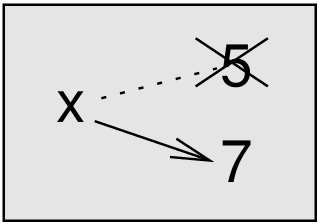
\includegraphics[width=0.7\linewidth]{images/chapter_7_1.png} % Ajusta el nombre del archivo
\caption{Diagrama de estado.}
\label{fig:diagrama_estado}
\end{figure}

\begin{lstlisting}
>>> a = 5
>>> b = a    # a and b are now equal
>>> a = 3    # a and b are no longer equal
>>> b
5
\end{lstlisting}

La tercera línea cambia el valor de \texttt{a} pero no cambia el valor de \texttt{b}, por lo que ya no son iguales.

Reasignar variables es a menudo útil, pero debes usarlo con precaución. Si los valores de las variables cambian frecuentemente, puede hacer que el código sea difícil de leer y depurar.

\section{Actualización de variables}

Un tipo común de reasignación es una \textbf{actualización}, donde el nuevo valor de la variable depende del anterior.

\begin{lstlisting}
>>> x = x + 1
\end{lstlisting}

Esto significa ``obtener el valor actual de \texttt{x}, agregar uno, y luego actualizar \texttt{x} con el nuevo valor.''

Si intentas actualizar una variable que no existe, obtienes un error, porque Python evalúa el lado derecho antes de asignar un valor a \texttt{x}:

\begin{lstlisting}
>>> x = x + 1
NameError: name 'x' is not defined
\end{lstlisting}

Antes de que puedas actualizar una variable, tienes que \textbf{inicializarla}, generalmente con una asignación simple:

\begin{lstlisting}
>>> x = 0
>>> x = x + 1
\end{lstlisting}

Actualizar una variable agregando 1 se llama un \textbf{incremento}; restar 1 se llama un \textbf{decremento}.

\section{La declaración \texttt{while}}

Las computadoras se usan a menudo para automatizar tareas repetitivas. Repetir tareas idénticas o similares sin cometer errores es algo que las computadoras hacen bien y las personas hacen mal. En un programa de computadora, la repetición también se llama \textbf{iteración}.

Ya hemos visto dos funciones, \texttt{countdown} y \texttt{print\_n}, que iteran usando recursión. Debido a que la iteración es tan común, Python proporciona características del lenguaje para hacerla más fácil. Una es la declaración \texttt{for} que vimos en la Sección 4.2. Volveremos a eso más tarde.

Otra es la declaración \texttt{while}. Aquí hay una versión de \texttt{countdown} que usa una declaración \texttt{while}:

\begin{lstlisting}
def countdown(n):
    while n > 0:
        print(n)
        n = n - 1
    print('Blastoff!')
\end{lstlisting}

Casi puedes leer la declaración \texttt{while} como si fuera inglés. Significa, ``Mientras \texttt{n} sea mayor que 0, muestra el valor de \texttt{n} y luego decrementa \texttt{n}. Cuando llegues a 0, muestra la palabra \texttt{Blastoff!}''

Más formalmente, aquí está el flujo de ejecución para una declaración \texttt{while}:

\begin{enumerate}
\item Determinar si la condición es verdadera o falsa.
\item Si es falsa, salir de la declaración \texttt{while} y continuar la ejecución en la siguiente declaración.
\item Si la condición es verdadera, ejecutar el cuerpo y luego volver al paso 1.
\end{enumerate}

Este tipo de flujo se llama un bucle porque el tercer paso se repite hacia el principio.

El cuerpo del bucle debe cambiar el valor de una o más variables para que la condición se vuelva falsa eventualmente y el bucle termine. De lo contrario, el bucle se repetirá para siempre, lo que se llama un \textbf{bucle infinito}. Una fuente inagotable de diversión para los científicos de la computación es la observación de que las instrucciones en el champú, ``Enjabonar, enjuagar, repetir'', son un bucle infinito.

En el caso de \texttt{countdown}, podemos probar que el bucle termina: si \texttt{n} es cero o negativo, el bucle nunca se ejecuta. De lo contrario, \texttt{n} se vuelve más pequeño cada vez a través del bucle, por lo que eventualmente tenemos que llegar a 0.

Para algunos otros bucles, no es tan fácil de decir. Por ejemplo:

\begin{lstlisting}
def sequence(n):
    while n != 1:
        print(n)
        if n % 2 == 0:        # n is even
            n = n / 2
        else:                 # n is odd
            n = n*3 + 1
\end{lstlisting}

La condición para este bucle es \texttt{n != 1}, por lo que el bucle continuará hasta que \texttt{n} sea 1, lo que hace que la condición sea falsa.

Cada vez a través del bucle, el programa muestra el valor de \texttt{n} y luego verifica si es par o impar. Si es par, \texttt{n} se divide por 2. Si es impar, el valor de \texttt{n} se reemplaza con \texttt{n*3 + 1}. Por ejemplo, si el argumento pasado a \texttt{sequence} es 3, los valores resultantes de \texttt{n} son 3, 10, 5, 16, 8, 4, 2, 1.

Dado que \texttt{n} a veces aumenta y a veces disminuye, no hay una prueba obvia de que \texttt{n} alguna vez llegue a 1, o que el programa termine. Para algunos valores particulares de \texttt{n}, podemos probar la terminación. Por ejemplo, si el valor inicial es una potencia de dos, \texttt{n} será par cada vez a través del bucle hasta que llegue a 1. El ejemplo anterior termina con una secuencia de este tipo, comenzando con 16.

La pregunta difícil es si podemos probar que este programa termina para \emph{todos} los valores positivos de \texttt{n}. Hasta ahora, nadie ha podido probarlo o refutarlo. (Ver \texttt{http://en.wikipedia.org/wiki/Collatz\_conjecture}.)

Como ejercicio, reescribe la función \texttt{print\_n} de la Sección 5.8 usando iteración en lugar de recursión.

\section{\texttt{break}}

A veces no sabes que es hora de terminar un bucle hasta que llegas a la mitad del cuerpo. En ese caso puedes usar la declaración \texttt{break} para saltar fuera del bucle.

Por ejemplo, supón que quieres recibir entrada del usuario hasta que escriban \texttt{done}. Podrías escribir:

\begin{lstlisting}
while True:
    line = input('> ')
    if line == 'done':
        break
    print(line)

print('Done!')
\end{lstlisting}

La condición del bucle es \texttt{True}, que siempre es verdadera, por lo que el bucle se ejecuta hasta que toca la declaración \texttt{break}.

Cada vez que pasa, solicita al usuario con un corchete angular. Si el usuario escribe \texttt{done}, la declaración \texttt{break} sale del bucle. De lo contrario, el programa repite lo que sea que el usuario escriba y vuelve al principio del bucle. Aquí hay una ejecución de muestra:

\begin{lstlisting}
> not done
not done
> done
Done!
\end{lstlisting}

Esta forma de escribir bucles \texttt{while} es común porque puedes verificar la condición en cualquier lugar del bucle (no solo al principio) y puedes expresar la condición de parada afirmativamente (``parar cuando esto suceda'') en lugar de negativamente (``seguir hasta que eso suceda'').

\subsection{Raíces cuadradas}

Los bucles se usan a menudo en programas que calculan resultados numéricos comenzando con una respuesta aproximada y mejorándola iterativamente.

Por ejemplo, una forma de calcular raíces cuadradas es el método de Newton. Supón que quieres conocer la raíz cuadrada de $a$. Si comienzas con casi cualquier estimación, $x$, puedes calcular una mejor estimación con la siguiente fórmula:

$$y = \frac{x + a/x}{2}$$

Por ejemplo, si $a$ es 4 y $x$ es 3:

\begin{lstlisting}
>>> a = 4
>>> x = 3
>>> y = (x + a/x) / 2
>>> y
2.1666666667
\end{lstlisting}

El resultado está más cerca de la respuesta correcta ($\sqrt{4} = 2$). Si repetimos el proceso con la nueva estimación, se acerca aún más:

\begin{lstlisting}
>>> x = y
>>> y = (x + a/x) / 2
>>> y
2.0064102564
\end{lstlisting}

Después de unas pocas actualizaciones más, la estimación es casi exacta:

\begin{lstlisting}
>>> x = y
>>> y = (x + a/x) / 2
>>> y
2.0001024003
>>> x = y
>>> y = (x + a/x) / 2
>>> y
2.0000000003
\end{lstlisting}

En general, no sabemos de antemano cuántos pasos toma llegar a la respuesta correcta, pero sabemos cuándo llegamos allí porque la estimación deja de cambiar:

\begin{lstlisting}
>>> x = y
>>> y = (x + a/x) / 2
>>> y
2.0
>>> x = y
>>> y = (x + a/x) / 2
>>> y
2.0
\end{lstlisting}

Cuando $y == x$, podemos parar. Aquí hay un bucle que comienza con una estimación inicial, $x$, y la mejora hasta que deja de cambiar:

\begin{lstlisting}
while True:
    print(x)
    y = (x + a/x) / 2
    if y == x:
        break
    x = y
\end{lstlisting}

Para la mayoría de los valores de $a$ esto funciona bien, pero en general es peligroso probar la igualdad de \texttt{float}. Los valores de punto flotante son solo aproximadamente correctos: la mayoría de los números racionales, como $1/3$, y los números irracionales, como $\sqrt{2}$, no se pueden representar exactamente con un \texttt{float}.

En lugar de verificar si $x$ y $y$ son exactamente iguales, es más seguro usar la función incorporada \texttt{abs} para calcular el valor absoluto, o magnitud, de la diferencia entre ellos:

\begin{lstlisting}
if abs(y-x) < epsilon:
    break
\end{lstlisting}

Donde \texttt{epsilon} tiene un valor como \texttt{0.0000001} que determina qué tan cerca es lo suficientemente cerca.

\section{Algoritmos}

El método de Newton es un ejemplo de un \textbf{algoritmo}: es un proceso mecánico para resolver una categoría de problemas (en este caso, calcular raíces cuadradas).

Para entender qué es un algoritmo, podría ayudar comenzar con algo que no es un algoritmo. Cuando aprendiste a multiplicar números de un solo dígito, probablemente memorizaste la tabla de multiplicación. En efecto, memorizaste 100 soluciones específicas. Ese tipo de conocimiento no es algorítmico.

Pero si fueras ``perezoso'', podrías haber aprendido algunos trucos. Por ejemplo, para encontrar el producto de $n$ y 9, puedes escribir $n - 1$ como el primer dígito y $10 - n$ como el segundo dígito. Este truco es una solución general para multiplicar cualquier número de un solo dígito por 9. ¡Eso es un algoritmo!

De manera similar, las técnicas que aprendiste para la suma con llevar, la resta con préstamo, y la división larga son todos algoritmos. Una de las características de los algoritmos es que no requieren ninguna inteligencia para ejecutarlos. Son procesos mecánicos donde cada paso sigue del último de acuerdo con un conjunto simple de reglas.

Ejecutar algoritmos es aburrido, pero diseñarlos es interesante, intelectualmente desafiante, y una parte central de la informática.

Algunas de las cosas que la gente hace naturalmente, sin dificultad o pensamiento consciente, son las más difíciles de expresar algorítmicamente. Entender el lenguaje natural es un buen ejemplo. Todos lo hacemos, pero hasta ahora nadie ha sido capaz de explicar \emph{cómo} lo hacemos, al menos no en la forma de un algoritmo.

\section{Depuración}

A medida que comiences a escribir programas más grandes, podrías encontrarte pasando más tiempo depurando. Más código significa más oportunidades de cometer errores y más lugares donde los bugs pueden esconderse.

Una forma de reducir tu tiempo de depuración es la ``depuración por bisección''. Por ejemplo, si hay 100 líneas en tu programa y las revisas una por una, tomaría 100 pasos.

En su lugar, trata de dividir el problema por la mitad. Busca el medio del programa, o cerca de él, un valor intermedio que puedas verificar. Agrega una declaración \texttt{print} (o algo más que tenga un efecto verificable) y ejecuta el programa.

Si la verificación del punto medio es incorrecta, debe haber un problema en la primera mitad del programa. Si es correcta, el problema está en la segunda mitad.

Cada vez que realizas una verificación como esta, reduces a la mitad el número de líneas que tienes que buscar. Después de seis pasos (que es menos de 100), estarías reducido a una o dos líneas de código, al menos en teoría.

En la práctica, no siempre está claro qué es el ``medio del programa'' y no siempre es posible verificarlo. No tiene sentido contar líneas y encontrar el punto medio exacto. En su lugar, piensa en lugares del programa donde podría haber errores y lugares donde es fácil poner una verificación. Luego elige un punto que divida el espacio de búsqueda aproximadamente por la mitad, ya sea que el bug esté antes o después de la verificación.

\section{Glosario}

\textbf{reasignación:} Asignar un nuevo valor a una variable que ya existe.

\textbf{actualización:} Una asignación donde el nuevo valor de la variable depende del valor anterior.

\textbf{inicialización:} Una asignación que da un valor inicial a una variable que será actualizada.

\textbf{incremento:} Una actualización que aumenta el valor de una variable (a menudo en uno).

\textbf{decremento:} Una actualización que disminuye el valor de una variable.

\textbf{iteración:} Ejecución repetida de un conjunto de declaraciones usando ya sea una llamada de función recursiva o un bucle.

\textbf{bucle infinito:} Un bucle en el cual la condición de terminación nunca se satisface.

\textbf{algoritmo:} Un proceso general para resolver una categoría de problemas.

\section{Ejercicios}

\textbf{Ejercicio 7.1.} Copia el bucle de la Sección 7.3 y encapsúlalo en una función llamada \texttt{mysqrt} que toma \texttt{a} como parámetro, elige un valor razonable de \texttt{x}, y devuelve una estimación de la raíz cuadrada de \texttt{a}.

Para probarlo, escribe una función llamada \texttt{test\_square\_root} que imprima una tabla como esta:

\begin{lstlisting}
a    mysqrt(a)     math.sqrt(a)  diff
-    ---------     ------------  ----
1.0  1.0           1.0           0.0
2.0  1.41421356237 1.41421356237 2.22044604925e-16
3.0  1.73205080757 1.73205080757 0.0
4.0  2.0           2.0           0.0
5.0  2.23606797775 2.23606797775 0.0
6.0  2.44948974278 2.44948974278 0.0
7.0  2.6457513110  2.6457513110  0.0
8.0  2.82842712475 2.82842712475 4.4408920985e-16
9.0  3.0           3.0           0.0
\end{lstlisting}

La primera columna es un número, \texttt{a}; la segunda columna es la raíz cuadrada de \texttt{a} calculada con \texttt{mysqrt}; la tercera columna es la raíz cuadrada calculada por \texttt{math.sqrt}; la cuarta columna es el valor absoluto de la diferencia entre las dos estimaciones.

\textbf{Ejercicio 7.2.} La función incorporada \texttt{eval} toma una cadena y la evalúa usando el intérprete de Python. Por ejemplo:

\begin{lstlisting}
>>> eval('1 + 2 * 3')
7
>>> import math
>>> eval('math.sqrt(5)')
2.2360679774997898
>>> eval('type(math.pi)')
<class 'float'>
\end{lstlisting}

Escribe una función llamada \texttt{eval\_loop} que iterativamente solicite al usuario, tome la entrada resultante y la evalúe usando \texttt{eval}, e imprima el resultado.

Debe continuar hasta que el usuario ingrese \texttt{'done'}, y luego devolver el valor de la última expresión que evaluó.

\vspace{1cm}

\textbf{Ejercicio 7.3.} El matemático Srinivasa Ramanujan encontró una serie infinita que puede ser usada para generar una aproximación numérica de $1/\pi$:

\begin{equation}
\frac{1}{\pi} = \frac{2\sqrt{2}}{9801} \sum_{k=0}^{\infty} \frac{(4k)!(1103+26390k)}{(k!)^4 396^{4k}}
\end{equation}

Escribe una función llamada \texttt{estimate\_pi} que use esta fórmula para calcular y devolver una estimación de $\pi$. Debe usar un bucle \texttt{while} para calcular términos de la sumatoria hasta que el último término sea menor que \texttt{1e-15} (que es la notación de Python para $10^{-15}$). Puedes verificar el resultado comparándolo con \texttt{math.pi}.

Solución: \texttt{https://thinkpython.com/code/pi.py}